\documentclass[12pt]{article}

\usepackage{fixltx2e}
\usepackage{textcomp}
\usepackage[cm]{fullpage}
\usepackage{amsfonts}
\usepackage{verbatim}
\usepackage[english]{babel}
\usepackage{pifont}
\usepackage{color}
\usepackage{setspace}
\usepackage{lscape}
\usepackage{indentfirst}
\usepackage[normalem]{ulem}
\usepackage{booktabs}
% \usepackage{nag}
\usepackage{natbib}
% \usepackage{bibtex}
\usepackage{float}
\usepackage{latexsym}
\usepackage{hyperref}
\usepackage{url}
% \usepackage{html}
\usepackage{epsfig}
\usepackage{graphicx}
\usepackage{amssymb}
\usepackage{amsmath}
\usepackage{bm}
\usepackage{array}
%\usepackage{mhchem}
\usepackage{ifthen}
\usepackage{caption}
\usepackage{xcolor}
\usepackage{amsthm}
\usepackage{amstext}
\usepackage{nicefrac}
\usepackage{algorithm}
\usepackage{algorithmic}
\usepackage[scientific-notation=true]{siunitx}
\usepackage{subfigure}
\usepackage[flushleft]{threeparttable}
\usepackage{lineno}
\usepackage{adjustbox}
\usepackage{ragged2e}
\usepackage{authblk}
\usepackage{multirow}
\usepackage[T1]{fontenc}

\setlength{\parskip}{1em}
\renewcommand{\baselinestretch}{2.0}
\renewcommand\Affilfont{\small}

\newcommand\ontop[2]{\genfrac{}{}{0pt}{}{#1}{#2}}

\begin{document}

\title{Supplementary figures and tables for StarBEAST2}
\author[1,2]{Huw A. Ogilvie\thanks{huw.ogilvie@anu.edu.au}}
\author[2,3]{Alexei J. Drummond}
\affil[1]{Division of Evolution, Ecology and Genetics, Research School of Biology, Australian National University, Canberra, Australia}
\affil[2]{Centre for Computational Evolution, University of Auckland, Auckland, New Zealand}
\affil[3]{Department of Computer Science, University of Auckland, Auckland, New Zealand}

\maketitle

\clearpage

\justifying

\begin{figure}[htb!]
\centering
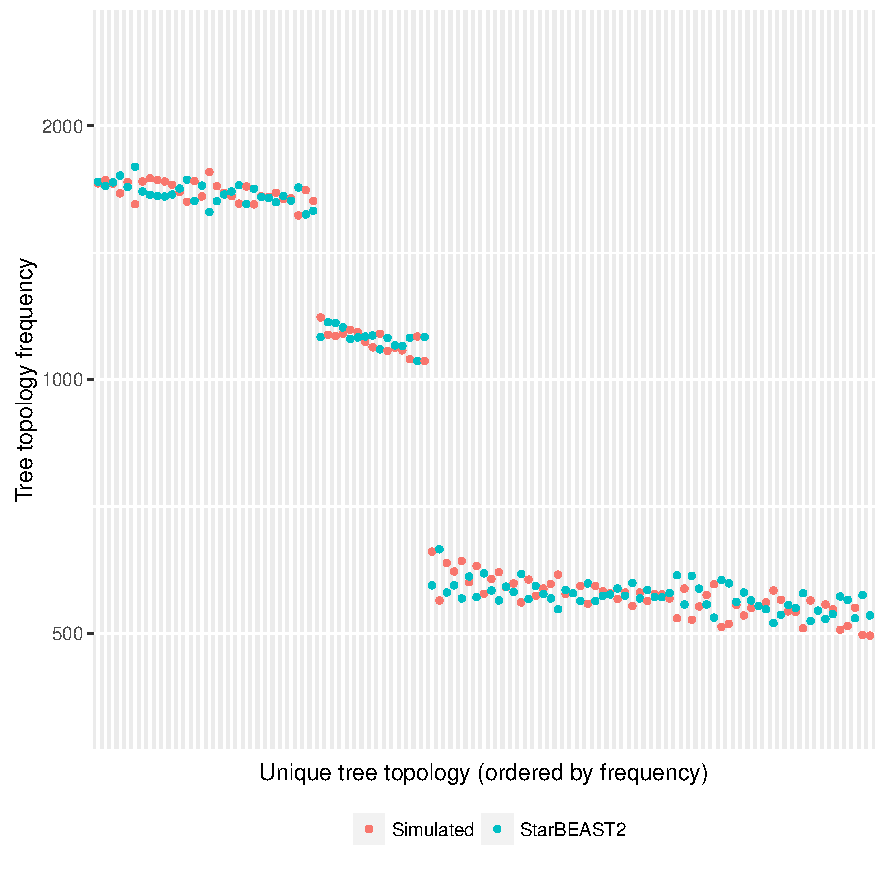
\includegraphics[width=16cm]{species_topology_frequencies.pdf}
\caption
{Frequency of five-taxon species tree topologies sampled from a birth-death prior
distribution. Topologies were sampled by simulating trees using biopy (red), or
by using a StarBEAST2 MCMC chain (blue). Frequencies are identical apart from
noise, indicating that StarBEAST2 is mathematically correct. Three levels of
probability are evident from left to right --- high probability balanced
topologies e.g. ((a,b),((c,d),e)), middle probability intermediate topologies
e.g. (((a,b),(c,d)),e), and low probability unbalanced topologies e.g.
((((a,b),c),d),e).}
\label{fig:speciesTopologyFrequencies}
\end{figure}

\clearpage

\begin{figure}[htb!]
\centering
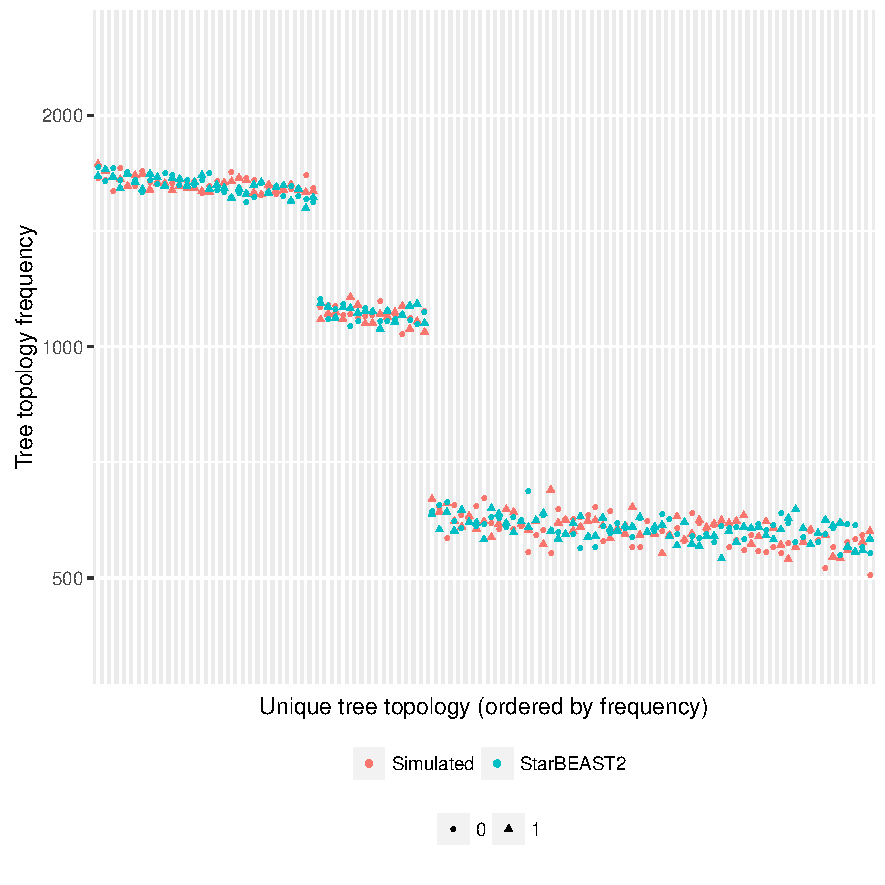
\includegraphics[width=16cm]{gene_topology_frequencies.pdf}
\caption
{Frequency of five-taxon gene tree topologies sampled from a multispecies
coalescent prior distribution. Topologies were sampled by simulating gene trees
within species trees using biopy (red), or by using a StarBEAST2 MCMC chain
(blue). Gene trees were sampled with two clock rates, 0.5 (circles) and 2.0
(triangles), although clock rate should not affect topology or node heights in
units of time. Frequencies are identical apart from noise, indicating that
StarBEAST2 is mathematically correct. Three levels of probability are evident
from left to right --- high probability balanced topologies e.g.
((a,b),((c,d),e)), middle probability intermediate topologies e.g.
(((a,b),(c,d)),e), and low probability unbalanced topologies e.g.
((((a,b),c),d),e).}
\label{fig:geneTopologyFrequencies}
\end{figure}

\clearpage

\begin{figure}[htb!]
\centering
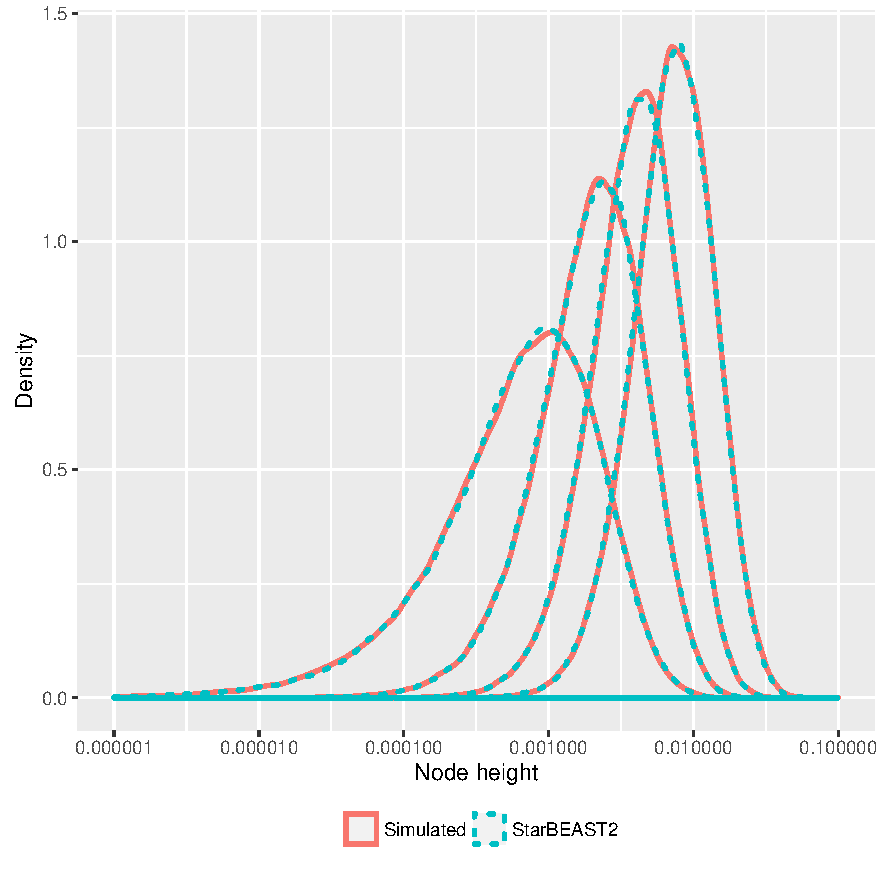
\includegraphics[width=16cm]{species_node_heights.pdf}
\caption
{Probability densities of five-taxon species tree node heights sampled from a
birth-death prior distribution. Node heights were sampled by simulating trees
using biopy (red), or by using a StarBEAST2 MCMC chain (blue). Probability
densities are plotted separately for each ranked node giving four peaks, one
for each internal node. Node height probability densities are identical apart
from noise, indicating that StarBEAST2 is mathematically correct.}
\label{fig:speciesNodeHeights}
\end{figure}

\clearpage

\begin{figure}[htb!]
\centering
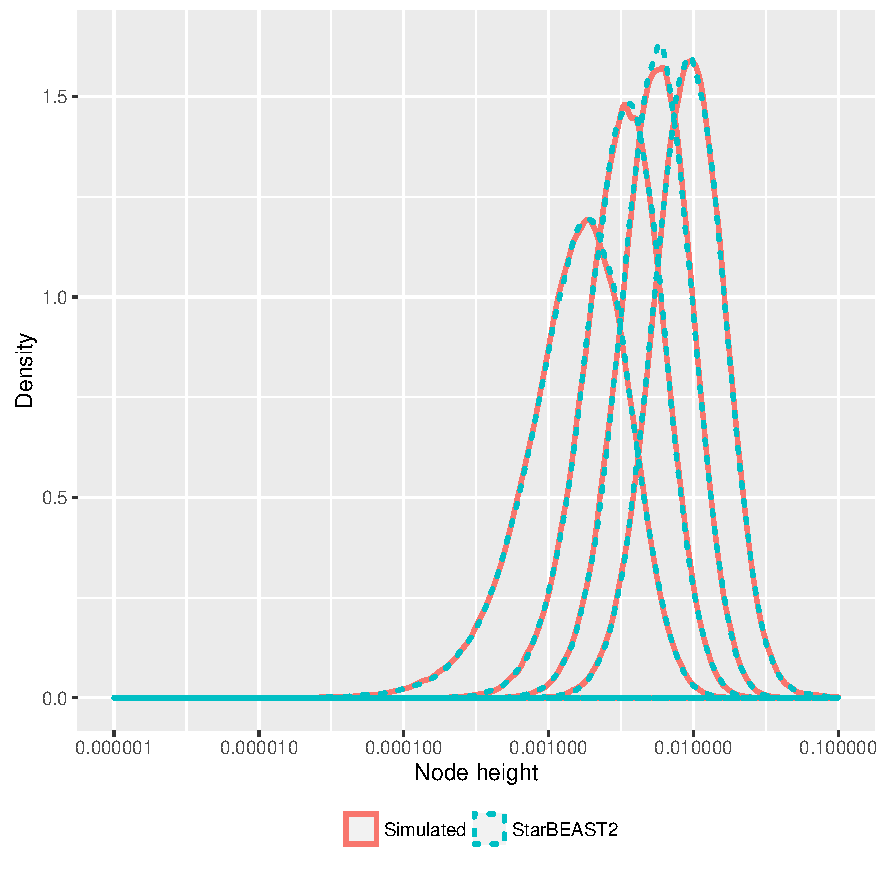
\includegraphics[width=16cm]{gene_node_heights.pdf}
\caption
{Probability densities of five-taxon gene tree node heights sampled from a
multispecies coalescent prior distribution. Node heights were sampled by
simulating gene trees within species trees using biopy (red), or by using a
StarBEAST2 MCMC chain (blue). Gene trees were sampled with two clock rates, 0.5
and 2.0, and node heights from both sets of gene trees were combined as clock
rate should not affect topology or node heights in units of time. Probability
densities are plotted separately for each ranked node giving four peaks, one for
each internal node. Node height probability densities are identical apart from
noise, indicating that StarBEAST2 is mathematically correct.}
\label{fig:geneNodeHeights}
\end{figure}

\clearpage

\begin{figure}[htb!]
\centering
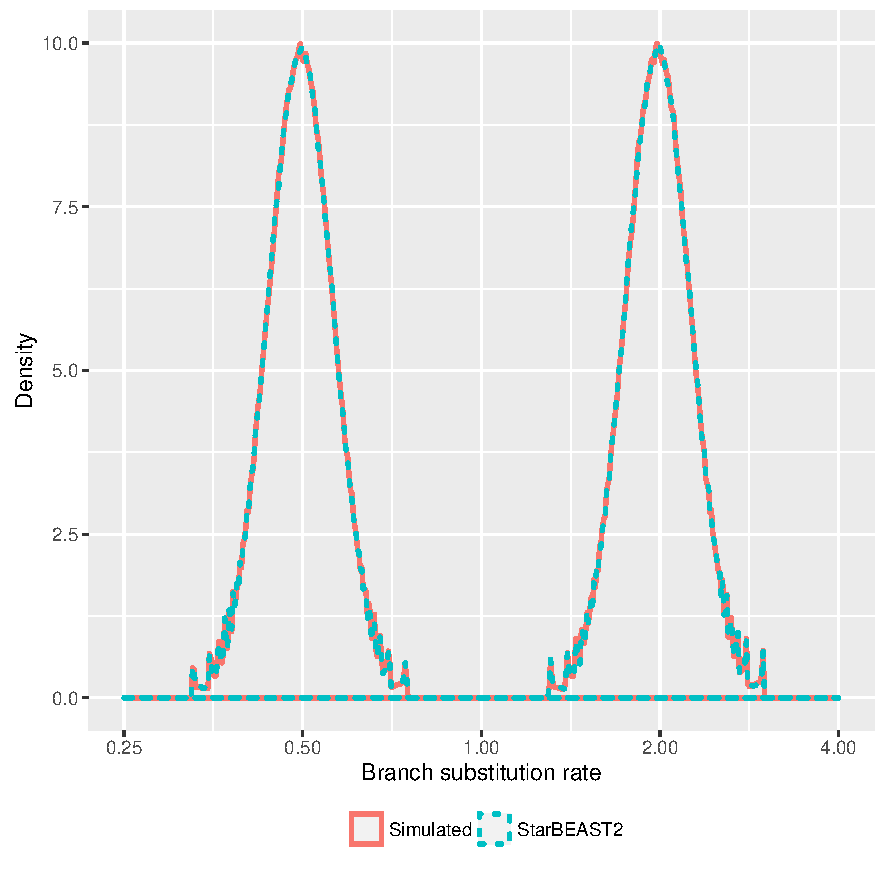
\includegraphics[width=16cm]{gene_branch_rates.pdf}
\caption
{Probability densities of five-taxon gene tree branch rates produced by a
species tree uncorrelated lognormal (UCLN) relaxed clock. Branch rates were
sampled by simulating gene trees within species trees using biopy and simulating
species tree branch rates using scipy (red), or by using a StarBEAST2 MCMC chain
(blue). Gene trees were sampled with two clock rates, 0.5 and 2.0, resulting in
two peaks. Branch rate probability densities are identical apart from noise,
indicating that StarBEAST2 is mathematically correct.}
\label{fig:geneBranchRatesUCLD}
\end{figure}

\begin{figure}[htb!]
\centering
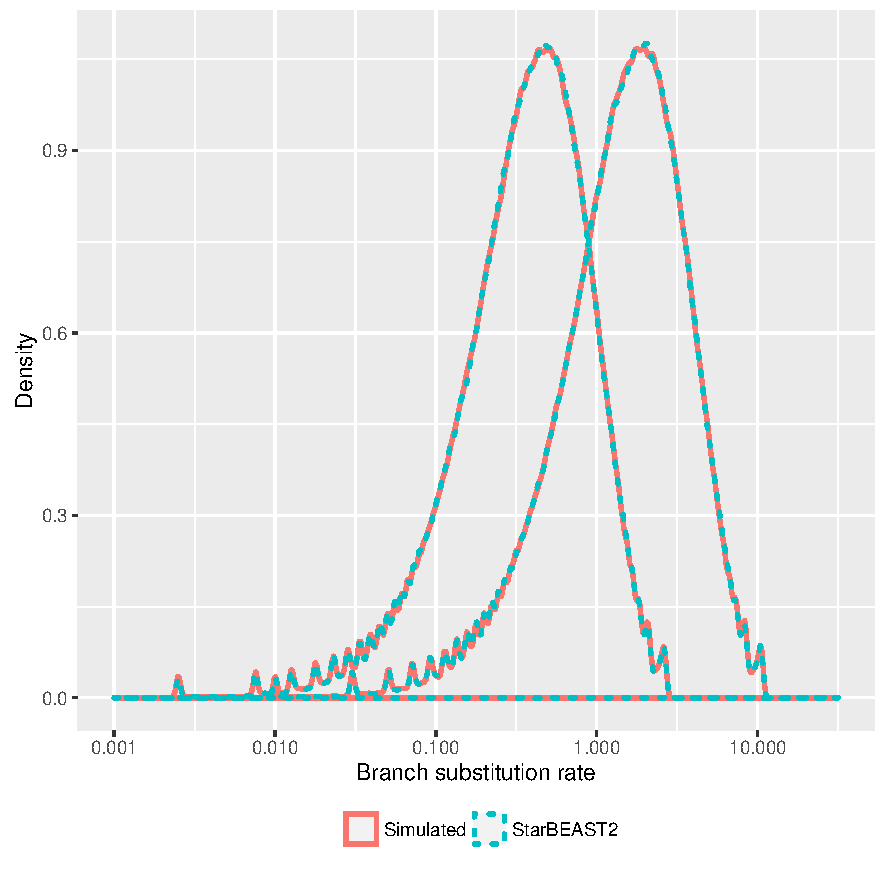
\includegraphics[width=16cm]{exp_gene_branch_rates.pdf}
\caption
{Probability densities of five-taxon gene tree branch rates produced by a
species tree uncorrelated exponential (UCED) relaxed clock. Branch rates were
sampled by simulating gene trees within species trees using biopy and simulating
species tree branch rates using scipy (red), or by using a StarBEAST2 MCMC chain
(blue). Gene trees were sampled with two clock rates, 0.5 and 2.0, resulting in
two peaks. Branch rate probability densities are identical apart from noise,
indicating that StarBEAST2 is mathematically correct.}
\label{fig:geneBranchRatesUCED}
\end{figure}

\clearpage

\begin{landscape}

\begin{table}[htb!]
\centering
\caption{Average ESS per hour convergence for \textit{Pseudacris} data.}
\label{tab:pseudacrisPerHour}
\begin{threeparttable}
\begin{adjustbox}{center}
\renewcommand{\arraystretch}{1.7}
\scriptsize
$\begin{array}{|c|c|c|c|c|c|c|c|c|c|c|c|c|}
\multicolumn{1}{c}{} & \multicolumn{1}{c}{\ontop{\text{Birth-death}}{\text{probability}}} & \multicolumn{1}{c}{\ontop{\text{Clock rate}}{\text{stdev}}} & \multicolumn{1}{c}{\ontop{\text{Extinction}}{\text{fraction}}} & \multicolumn{1}{c}{\ontop{\text{Among-site}}{\text{rate variation}}} & \multicolumn{1}{c}{\ontop{\text{Transition/}}{\text{Transversion}} \kappa} & \multicolumn{1}{c}{\ontop{\text{Phylogenetic}}{\text{likelihood}}} & \multicolumn{1}{c}{\ontop{\text{Diversification}}{\text{rate}}} & \multicolumn{1}{c}{\ontop{\text{Population}}{\text{Mean}}} & \multicolumn{1}{c}{\text{Log-posterior}} & \multicolumn{1}{c}{\text{Log-prior}} & \multicolumn{1}{c}{\ontop{\text{Species}}{\text{tree height}}} & \multicolumn{1}{c}{\ontop{\text{Coalescent}}{\text{probability}}}\tabularnewline
\hline
\lozenge\lozenge\lozenge\lozenge & \ontop{81.2}{72.8 - 91.2} & \ontop{191.9}{156.1 - 228.1} & \ontop{175.7}{150.3 - 201.4} & \ontop{213.0}{166.5 - 260.5} & \ontop{232.1}{174.1 - 287.3} & \ontop{19.3}{17.2 - 22.2} & \ontop{180.9}{153.0 - 209.3} & \ontop{26.2}{23.9 - 28.4} & \ontop{21.5}{19.4 - 23.7} & \ontop{29.0}{26.7 - 31.3} & \ontop{9.0}{7.1 - 10.8} & \ontop{18.7}{16.9 - 20.3}\tabularnewline
\hline
\lozenge\lozenge\lozenge\blacklozenge & \ontop{120.9}{110.1 - 130.7} & \ontop{245.8}{220.3 - 276.1} & \ontop{207.2}{195.5 - 220.9} & \ontop{366.5}{300.2 - 442.5} & \ontop{379.4}{311.1 - 458.7} & \ontop{27.1}{23.6 - 32.1} & \ontop{217.5}{205.7 - 232.8} & \ontop{35.7}{32.9 - 38.9} & \ontop{30.1}{27.8 - 32.5} & \ontop{32.5}{29.7 - 35.8} & \ontop{20.2}{17.6 - 23.1} & \ontop{24.6}{22.6 - 26.8}\tabularnewline
\hline
\lozenge\lozenge\blacklozenge\lozenge & \ontop{65.2}{59.4 - 70.4} & \ontop{129.0}{112.8 - 150.7} & \ontop{131.7}{115.6 - 152.6} & \ontop{154.3}{125.1 - 190.6} & \ontop{154.7}{124.8 - 195.2} & \ontop{17.2}{15.4 - 18.9} & \ontop{129.5}{110.9 - 153.8} & \ontop{19.8}{18.1 - 22.0} & \ontop{16.3}{14.5 - 18.5} & \ontop{23.8}{22.2 - 25.9} & \ontop{7.0}{5.6 - 8.6} & \ontop{14.4}{13.0 - 15.8}\tabularnewline
\hline
\lozenge\lozenge\blacklozenge\blacklozenge & \ontop{89.7}{82.9 - 96.6} & \ontop{191.0}{176.5 - 212.4} & \ontop{174.1}{168.9 - 181.2} & \ontop{257.0}{225.1 - 318.4} & \ontop{270.2}{237.7 - 333.6} & \ontop{23.3}{21.6 - 26.6} & \ontop{175.6}{170.8 - 184.9} & \ontop{28.0}{25.5 - 31.0} & \ontop{23.2}{21.1 - 25.6} & \ontop{28.9}{25.8 - 31.9} & \ontop{14.1}{12.3 - 16.4} & \ontop{19.2}{17.5 - 21.0}\tabularnewline
\hline
\lozenge\blacklozenge\lozenge\lozenge & \ontop{30.8}{26.5 - 35.9} & \ontop{54.0}{49.2 - 66.8} & \ontop{53.5}{48.2 - 67.2} & \ontop{55.5}{50.1 - 69.6} & \ontop{54.9}{49.2 - 70.0} & \ontop{11.6}{10.7 - 12.7} & \ontop{54.6}{47.7 - 67.6} & \ontop{18.9}{17.7 - 20.1} & \ontop{15.8}{14.5 - 16.9} & \ontop{17.3}{16.1 - 18.4} & \ontop{2.7}{2.3 - 3.1} & \ontop{14.2}{13.2 - 15.3}\tabularnewline
\hline
\lozenge\blacklozenge\lozenge\blacklozenge & \ontop{59.9}{53.8 - 66.4} & \ontop{121.7}{100.1 - 144.9} & \ontop{109.3}{92.9 - 126.7} & \ontop{135.6}{106.0 - 164.5} & \ontop{137.5}{106.3 - 167.9} & \ontop{18.1}{16.6 - 19.6} & \ontop{107.5}{92.1 - 123.9} & \ontop{24.7}{22.7 - 26.7} & \ontop{22.4}{20.9 - 24.1} & \ontop{23.0}{21.2 - 24.7} & \ontop{6.0}{5.0 - 7.4} & \ontop{17.8}{16.7 - 18.8}\tabularnewline
\hline
\lozenge\blacklozenge\blacklozenge\lozenge & \ontop{31.9}{26.8 - 37.8} & \ontop{64.6}{50.6 - 78.7} & \ontop{62.5}{50.2 - 75.4} & \ontop{66.0}{52.2 - 81.2} & \ontop{65.8}{52.6 - 81.9} & \ontop{10.2}{9.0 - 11.4} & \ontop{61.7}{49.8 - 74.6} & \ontop{16.2}{15.2 - 17.6} & \ontop{13.0}{11.9 - 14.4} & \ontop{15.6}{14.2 - 16.9} & \ontop{2.7}{2.2 - 3.4} & \ontop{11.7}{10.8 - 12.9}\tabularnewline
\hline
\lozenge\blacklozenge\blacklozenge\blacklozenge & \ontop{49.1}{46.2 - 54.4} & \ontop{100.3}{80.8 - 123.3} & \ontop{91.6}{79.7 - 105.8} & \ontop{112.8}{86.8 - 148.1} & \ontop{114.6}{86.9 - 150.5} & \ontop{15.9}{14.7 - 17.0} & \ontop{90.6}{75.5 - 108.6} & \ontop{21.9}{20.2 - 23.8} & \ontop{20.5}{19.2 - 22.2} & \ontop{20.5}{19.3 - 21.5} & \ontop{5.1}{4.3 - 6.3} & \ontop{16.8}{15.8 - 18.1}\tabularnewline
\hline
\blacklozenge\lozenge\lozenge\lozenge & \ontop{105.1}{97.4 - 114.0} & \ontop{179.9}{150.4 - 215.8} & \ontop{172.4}{150.7 - 196.7} & \ontop{203.2}{164.5 - 247.6} & \ontop{207.8}{166.8 - 258.0} & \ontop{23.5}{19.1 - 28.1} & \ontop{176.8}{155.9 - 202.8} & \ontop{44.9}{41.0 - 49.0} & \ontop{30.3}{27.8 - 33.7} & \ontop{148.8}{132.9 - 171.5} & \ontop{10.2}{8.9 - 11.9} & \ontop{29.2}{27.5 - 31.7}\tabularnewline
\hline
\blacklozenge\lozenge\lozenge\blacklozenge & \ontop{128.1}{119.1 - 136.7} & \ontop{264.8}{235.3 - 293.6} & \ontop{217.5}{207.0 - 227.5} & \ontop{437.7}{363.1 - 520.4} & \ontop{473.2}{395.8 - 569.7} & \ontop{33.4}{30.4 - 36.5} & \ontop{223.4}{210.0 - 241.9} & \ontop{69.0}{63.3 - 74.9} & \ontop{48.1}{43.5 - 52.6} & \ontop{200.9}{187.6 - 217.3} & \ontop{25.9}{20.0 - 32.6} & \ontop{38.9}{35.0 - 42.6}\tabularnewline
\hline
\blacklozenge\lozenge\blacklozenge\lozenge & \ontop{79.9}{70.7 - 88.2} & \ontop{140.5}{114.8 - 167.4} & \ontop{138.4}{116.6 - 159.1} & \ontop{167.5}{125.2 - 212.7} & \ontop{167.5}{122.3 - 220.7} & \ontop{18.9}{16.0 - 23.3} & \ontop{136.6}{115.2 - 159.9} & \ontop{35.8}{32.1 - 40.1} & \ontop{24.3}{21.4 - 27.1} & \ontop{117.7}{97.9 - 140.5} & \ontop{7.5}{6.0 - 9.8} & \ontop{21.6}{19.0 - 23.9}\tabularnewline
\hline
\blacklozenge\lozenge\blacklozenge\blacklozenge & \ontop{106.3}{99.9 - 112.2} & \ontop{226.2}{208.5 - 240.0} & \ontop{188.6}{177.7 - 198.6} & \ontop{396.3}{332.9 - 425.9} & \ontop{433.8}{366.2 - 463.6} & \ontop{30.3}{27.3 - 34.3} & \ontop{196.8}{186.8 - 207.1} & \ontop{63.5}{55.5 - 70.9} & \ontop{42.8}{38.3 - 47.5} & \ontop{174.1}{162.5 - 188.2} & \ontop{22.8}{18.9 - 26.6} & \ontop{35.7}{32.5 - 39.3}\tabularnewline
\hline
\blacklozenge\blacklozenge\lozenge\lozenge & \ontop{34.0}{27.9 - 42.6} & \ontop{56.8}{47.6 - 76.5} & \ontop{55.8}{48.1 - 71.2} & \ontop{56.2}{47.3 - 76.0} & \ontop{57.4}{47.9 - 78.4} & \ontop{13.9}{12.0 - 15.8} & \ontop{55.6}{47.7 - 72.1} & \ontop{29.6}{26.6 - 33.1} & \ontop{22.5}{20.5 - 25.7} & \ontop{48.0}{41.2 - 62.0} & \ontop{2.6}{2.2 - 3.4} & \ontop{20.7}{18.7 - 22.6}\tabularnewline
\hline
\blacklozenge\blacklozenge\lozenge\blacklozenge & \ontop{70.0}{63.9 - 76.9} & \ontop{132.9}{111.2 - 161.9} & \ontop{119.1}{103.1 - 134.7} & \ontop{153.7}{124.1 - 207.5} & \ontop{155.3}{125.2 - 213.7} & \ontop{20.7}{19.0 - 23.3} & \ontop{118.6}{101.7 - 134.3} & \ontop{46.3}{43.2 - 49.9} & \ontop{36.0}{33.9 - 38.5} & \ontop{114.0}{96.3 - 135.6} & \ontop{6.1}{5.4 - 7.7} & \ontop{30.8}{29.2 - 32.4}\tabularnewline
\hline
\blacklozenge\blacklozenge\blacklozenge\lozenge & \ontop{30.4}{25.9 - 37.4} & \ontop{56.2}{43.1 - 80.4} & \ontop{54.3}{43.8 - 71.5} & \ontop{56.7}{45.0 - 79.3} & \ontop{58.9}{44.0 - 83.3} & \ontop{12.9}{11.7 - 14.0} & \ontop{55.0}{43.1 - 76.2} & \ontop{26.3}{23.8 - 30.3} & \ontop{19.0}{17.0 - 21.2} & \ontop{47.0}{39.3 - 59.9} & \ontop{2.5}{2.0 - 3.4} & \ontop{16.9}{15.3 - 19.0}\tabularnewline
\hline
\blacklozenge\blacklozenge\blacklozenge\blacklozenge & \ontop{60.5}{54.2 - 65.7} & \ontop{110.2}{91.4 - 128.6} & \ontop{101.1}{87.7 - 115.9} & \ontop{124.0}{99.5 - 149.4} & \ontop{126.9}{102.6 - 151.6} & \ontop{18.9}{17.7 - 20.3} & \ontop{97.9}{84.8 - 112.7} & \ontop{41.4}{38.7 - 44.1} & \ontop{32.1}{30.1 - 34.3} & \ontop{94.9}{79.2 - 111.3} & \ontop{5.2}{4.6 - 6.1} & \ontop{27.0}{25.3 - 28.8}\tabularnewline
\hline
\end{array}$
\end{adjustbox}
\begin{tablenotes}
\scriptsize
\item Top numbers show trimmed means (25\% trim was applied to reduce the influence of outliers)
\item Bottom numbers show 95\% confidence intervals for the trimmed mean calculated by bootstrapping
\item Filled diamonds indicate which new features are enabled. From left-to-right; analytical integration of population sizes, species tree relaxed clocks, coordinated topology operators, and coordinated height operators.
\end{tablenotes}
\end{threeparttable}
\end{table}

\clearpage

\begin{table}[htb!]
\centering
\caption{Average ESS per million states convergence for \textit{Pseudacris} data.}
\label{tab:pseudacrisPerMstates}
\begin{threeparttable}
\begin{adjustbox}{center}
\renewcommand{\arraystretch}{1.7}
\scriptsize
$\begin{array}{|c|c|c|c|c|c|c|c|c|c|c|c|c|}
\multicolumn{1}{c}{} & \multicolumn{1}{c}{\ontop{\text{Birth-death}}{\text{probability}}} & \multicolumn{1}{c}{\ontop{\text{Clock rate}}{\text{stdev}}} & \multicolumn{1}{c}{\ontop{\text{Extinction}}{\text{fraction}}} & \multicolumn{1}{c}{\ontop{\text{Among-site}}{\text{rate variation}}} & \multicolumn{1}{c}{\ontop{\text{Transition/}}{\text{Transversion}} \kappa} & \multicolumn{1}{c}{\ontop{\text{Phylogenetic}}{\text{likelihood}}} & \multicolumn{1}{c}{\ontop{\text{Diversification}}{\text{rate}}} & \multicolumn{1}{c}{\ontop{\text{Population}}{\text{Mean}}} & \multicolumn{1}{c}{\text{Log-posterior}} & \multicolumn{1}{c}{\text{Log-prior}} & \multicolumn{1}{c}{\ontop{\text{Species}}{\text{tree height}}} & \multicolumn{1}{c}{\ontop{\text{Coalescent}}{\text{probability}}}\tabularnewline
\hline
\lozenge\lozenge\lozenge\lozenge & \ontop{7.29}{6.44 - 8.14} & \ontop{17.20}{13.99 - 20.42} & \ontop{15.75}{13.52 - 18.22} & \ontop{19.04}{14.92 - 23.59} & \ontop{20.83}{15.56 - 26.52} & \ontop{1.72}{1.53 - 1.97} & \ontop{16.21}{13.69 - 18.82} & \ontop{2.36}{2.14 - 2.56} & \ontop{1.94}{1.74 - 2.14} & \ontop{2.61}{2.44 - 2.79} & \ontop{0.81}{0.65 - 0.96} & \ontop{1.68}{1.52 - 1.85}\tabularnewline
\hline
\lozenge\lozenge\lozenge\blacklozenge & \ontop{12.41}{11.35 - 13.43} & \ontop{25.19}{22.43 - 28.37} & \ontop{21.38}{20.22 - 22.81} & \ontop{37.90}{30.64 - 45.15} & \ontop{39.27}{31.81 - 46.79} & \ontop{2.79}{2.43 - 3.23} & \ontop{22.38}{21.16 - 24.00} & \ontop{3.66}{3.34 - 3.99} & \ontop{3.08}{2.85 - 3.36} & \ontop{3.35}{3.04 - 3.67} & \ontop{2.07}{1.80 - 2.38} & \ontop{2.52}{2.32 - 2.73}\tabularnewline
\hline
\lozenge\lozenge\blacklozenge\lozenge & \ontop{7.43}{6.74 - 8.06} & \ontop{14.59}{12.68 - 17.26} & \ontop{15.00}{13.17 - 17.46} & \ontop{17.43}{14.18 - 21.57} & \ontop{17.62}{14.10 - 22.16} & \ontop{1.96}{1.74 - 2.15} & \ontop{14.72}{12.62 - 17.31} & \ontop{2.25}{2.08 - 2.48} & \ontop{1.86}{1.64 - 2.11} & \ontop{2.71}{2.52 - 2.94} & \ontop{0.79}{0.64 - 0.99} & \ontop{1.63}{1.47 - 1.79}\tabularnewline
\hline
\lozenge\lozenge\blacklozenge\blacklozenge & \ontop{10.88}{10.11 - 11.71} & \ontop{23.12}{21.38 - 25.45} & \ontop{21.06}{20.50 - 21.77} & \ontop{31.02}{27.42 - 38.29} & \ontop{32.84}{28.80 - 40.27} & \ontop{2.83}{2.60 - 3.26} & \ontop{21.29}{20.79 - 22.39} & \ontop{3.38}{3.11 - 3.75} & \ontop{2.80}{2.53 - 3.09} & \ontop{3.50}{3.18 - 3.85} & \ontop{1.71}{1.51 - 2.00} & \ontop{2.33}{2.13 - 2.54}\tabularnewline
\hline
\lozenge\blacklozenge\lozenge\lozenge & \ontop{4.58}{3.90 - 5.33} & \ontop{8.02}{7.29 - 9.94} & \ontop{7.94}{7.17 - 9.94} & \ontop{8.23}{7.45 - 10.21} & \ontop{8.17}{7.34 - 10.38} & \ontop{1.72}{1.58 - 1.87} & \ontop{8.08}{7.16 - 9.98} & \ontop{2.80}{2.64 - 2.99} & \ontop{2.34}{2.13 - 2.51} & \ontop{2.56}{2.40 - 2.73} & \ontop{0.39}{0.34 - 0.45} & \ontop{2.11}{1.97 - 2.25}\tabularnewline
\hline
\lozenge\blacklozenge\lozenge\blacklozenge & \ontop{9.72}{8.79 - 10.62} & \ontop{19.72}{16.21 - 23.69} & \ontop{17.74}{15.23 - 20.54} & \ontop{22.02}{17.81 - 27.04} & \ontop{22.32}{17.30 - 27.41} & \ontop{2.94}{2.70 - 3.18} & \ontop{17.51}{15.06 - 20.30} & \ontop{4.01}{3.67 - 4.37} & \ontop{3.65}{3.40 - 3.90} & \ontop{3.74}{3.41 - 3.99} & \ontop{0.98}{0.80 - 1.21} & \ontop{2.89}{2.74 - 3.07}\tabularnewline
\hline
\lozenge\blacklozenge\blacklozenge\lozenge & \ontop{5.68}{4.72 - 6.70} & \ontop{11.48}{9.35 - 14.10} & \ontop{11.11}{8.92 - 13.43} & \ontop{11.73}{9.23 - 14.46} & \ontop{11.71}{9.28 - 14.52} & \ontop{1.82}{1.62 - 2.04} & \ontop{10.96}{8.86 - 13.24} & \ontop{2.88}{2.69 - 3.16} & \ontop{2.31}{2.12 - 2.54} & \ontop{2.77}{2.53 - 3.03} & \ontop{0.48}{0.38 - 0.59} & \ontop{2.09}{1.94 - 2.27}\tabularnewline
\hline
\lozenge\blacklozenge\blacklozenge\blacklozenge & \ontop{9.17}{8.62 - 10.02} & \ontop{18.70}{15.25 - 23.42} & \ontop{17.02}{14.64 - 19.80} & \ontop{20.96}{15.55 - 28.53} & \ontop{21.33}{16.89 - 28.54} & \ontop{2.96}{2.71 - 3.15} & \ontop{16.90}{14.10 - 20.11} & \ontop{4.07}{3.78 - 4.42} & \ontop{3.82}{3.58 - 4.13} & \ontop{3.80}{3.59 - 3.98} & \ontop{0.94}{0.81 - 1.19} & \ontop{3.15}{2.94 - 3.36}\tabularnewline
\hline
\blacklozenge\lozenge\lozenge\lozenge & \ontop{9.68}{9.02 - 10.59} & \ontop{16.72}{13.98 - 19.85} & \ontop{15.99}{13.95 - 18.27} & \ontop{18.78}{15.24 - 22.97} & \ontop{19.20}{15.07 - 23.60} & \ontop{2.17}{1.76 - 2.56} & \ontop{16.43}{14.42 - 18.71} & \ontop{4.14}{3.79 - 4.55} & \ontop{2.80}{2.56 - 3.08} & \ontop{13.76}{12.31 - 15.77} & \ontop{0.94}{0.84 - 1.08} & \ontop{2.69}{2.54 - 2.92}\tabularnewline
\hline
\blacklozenge\lozenge\lozenge\blacklozenge & \ontop{13.56}{12.60 - 14.40} & \ontop{27.89}{24.74 - 30.89} & \ontop{22.93}{21.73 - 23.93} & \ontop{46.06}{38.22 - 55.35} & \ontop{49.79}{41.54 - 59.48} & \ontop{3.53}{3.20 - 3.84} & \ontop{23.58}{22.19 - 25.52} & \ontop{7.26}{6.66 - 7.89} & \ontop{5.06}{4.62 - 5.53} & \ontop{21.23}{19.72 - 22.70} & \ontop{2.72}{2.09 - 3.42} & \ontop{4.08}{3.71 - 4.47}\tabularnewline
\hline
\blacklozenge\lozenge\blacklozenge\lozenge & \ontop{9.28}{8.22 - 10.26} & \ontop{16.30}{13.28 - 19.30} & \ontop{16.08}{13.55 - 18.38} & \ontop{19.41}{14.78 - 24.43} & \ontop{19.39}{14.40 - 25.83} & \ontop{2.20}{1.89 - 2.66} & \ontop{15.89}{13.52 - 18.77} & \ontop{4.19}{3.76 - 4.67} & \ontop{2.82}{2.48 - 3.14} & \ontop{13.65}{11.57 - 16.18} & \ontop{0.87}{0.70 - 1.15} & \ontop{2.51}{2.23 - 2.76}\tabularnewline
\hline
\blacklozenge\lozenge\blacklozenge\blacklozenge & \ontop{13.12}{12.25 - 13.92} & \ontop{27.94}{25.70 - 29.64} & \ontop{23.19}{21.88 - 24.46} & \ontop{48.66}{41.67 - 52.01} & \ontop{53.59}{45.38 - 56.30} & \ontop{3.73}{3.38 - 4.20} & \ontop{24.28}{23.07 - 25.59} & \ontop{7.76}{6.82 - 8.60} & \ontop{5.24}{4.75 - 5.83} & \ontop{21.44}{20.11 - 22.94} & \ontop{2.80}{2.33 - 3.21} & \ontop{4.39}{3.99 - 4.79}\tabularnewline
\hline
\blacklozenge\blacklozenge\lozenge\lozenge & \ontop{5.16}{4.20 - 6.51} & \ontop{8.61}{7.31 - 11.33} & \ontop{8.47}{7.31 - 10.86} & \ontop{8.56}{7.20 - 11.07} & \ontop{8.75}{7.31 - 11.50} & \ontop{2.12}{1.83 - 2.41} & \ontop{8.46}{7.28 - 10.57} & \ontop{4.51}{4.07 - 5.03} & \ontop{3.43}{3.11 - 3.81} & \ontop{7.29}{6.38 - 9.57} & \ontop{0.40}{0.33 - 0.52} & \ontop{3.15}{2.86 - 3.44}\tabularnewline
\hline
\blacklozenge\blacklozenge\lozenge\blacklozenge & \ontop{11.65}{10.58 - 12.94} & \ontop{22.04}{18.30 - 26.42} & \ontop{19.77}{16.80 - 22.50} & \ontop{25.52}{20.52 - 33.87} & \ontop{25.76}{20.43 - 33.86} & \ontop{3.44}{3.17 - 3.87} & \ontop{19.69}{16.81 - 22.29} & \ontop{7.69}{7.16 - 8.31} & \ontop{5.97}{5.61 - 6.38} & \ontop{18.90}{16.29 - 22.27} & \ontop{1.02}{0.90 - 1.23} & \ontop{5.11}{4.86 - 5.40}\tabularnewline
\hline
\blacklozenge\blacklozenge\blacklozenge\lozenge & \ontop{5.54}{4.70 - 6.79} & \ontop{10.19}{7.86 - 14.22} & \ontop{9.88}{7.85 - 13.19} & \ontop{10.30}{8.17 - 14.45} & \ontop{10.69}{8.01 - 15.51} & \ontop{2.36}{2.15 - 2.57} & \ontop{9.99}{7.82 - 13.53} & \ontop{4.79}{4.35 - 5.45} & \ontop{3.46}{3.09 - 3.90} & \ontop{8.57}{7.19 - 11.01} & \ontop{0.45}{0.36 - 0.61} & \ontop{3.07}{2.77 - 3.45}\tabularnewline
\hline
\blacklozenge\blacklozenge\blacklozenge\blacklozenge & \ontop{11.44}{10.31 - 12.65} & \ontop{20.88}{17.25 - 24.53} & \ontop{19.17}{16.41 - 21.95} & \ontop{23.53}{19.14 - 28.65} & \ontop{24.06}{19.18 - 28.90} & \ontop{3.59}{3.37 - 3.89} & \ontop{18.55}{16.18 - 21.15} & \ontop{7.89}{7.38 - 8.37} & \ontop{6.09}{5.68 - 6.56} & \ontop{17.95}{14.81 - 21.09} & \ontop{0.99}{0.86 - 1.15} & \ontop{5.12}{4.79 - 5.49}\tabularnewline
\hline
\end{array}$
\end{adjustbox}
\begin{tablenotes}
\scriptsize
\item Top numbers show trimmed means (25\% trim was applied to reduce the influence of outliers)
\item Bottom numbers show 95\% confidence intervals for the trimmed mean calculated by bootstrapping
\item Filled diamonds indicate which new features are enabled. From left-to-right; analytical integration of population sizes, species tree relaxed clocks, coordinated topology operators, and coordinated height operators.
\end{tablenotes}
\end{threeparttable}
\end{table}

\clearpage

\begin{table}[htb!]
\centering
\caption{Average ESS per hour convergence for simulated data.}
\label{tab:simulatedPerHour}
\begin{threeparttable}
\begin{adjustbox}{center}
\renewcommand{\arraystretch}{1.2}
\footnotesize
\begin{tabular}{|c|c|c|c|c|c|}
\multicolumn{1}{c}{Statistic} & \multicolumn{1}{c}{Concatenation} & \multicolumn{1}{c}{Concatenation 10X} & \multicolumn{1}{c}{*BEAST} & \multicolumn{1}{c}{StarBEAST2 GT-UCLN} & \multicolumn{1}{c}{StarBEAST2 ST-UCLN}\tabularnewline
\hline
Net diversification rate & 1094.2 (1043.9--1149.2) & 94.7 (90.7--98.5) & 137.2 (118.8--155.8) & 219.5 (201.7--233.1) & 139.6 (117.0--159.9)\tabularnewline
\hline
Species tree height & 1217.8 (1092.7--1358.3) & 16.4 (14.0--19.1) & 6.7 (5.7--7.9) & 19.3 (16.0--23.6) & 9.8 (7.6--12.3)\tabularnewline
\hline
Log-posterior & 747.0 (719.1--777.7) & 7.7 (7.3--8.1) & 18.2 (16.1--20.3) & 45.6 (40.3--51.1) & 34.9 (31.7--38.7)\tabularnewline
\hline
Clock rates $\sigma$ & 1490.1 (1379.4--1589.5) & 45.7 (43.9--47.7) & 139.6 (122.7--160.2) & 235.9 (212.9--257.5) & 163.1 (136.2--189.4)\tabularnewline
\hline
Coalescent probability & NA & NA & 16.3 (14.5--18.2) & 41.7 (36.7--46.2) & 31.4 (28.2--34.8)\tabularnewline
\hline
Phylogenetic likelihood & 739.4 (705.2--769.6) & 7.5 (7.1--7.9) & 45.6 (41.6--50.8) & 86.2 (79.9--93.2) & 53.7 (47.7--59.0)\tabularnewline
\hline
Birth-death probability & 1259.3 (1152.2--1387.2) & 32.7 (29.9--35.9) & 76.7 (70.2--85.0) & 136.6 (125.4--148.6) & 92.5 (78.3--105.6)\tabularnewline
\hline
Substitution model $\kappa$ & 5019.1 (4768.8--5233.1) & 150.7 (145.3--157.2) & 154.5 (133.0--182.4) & 448.5 (365.2--522.9) & 241.6 (185.9--307.6)\tabularnewline
\hline
Substitution model $\alpha$ & 2329.4 (2159.0--2532.9) & 139.5 (133.7--147.4) & 150.2 (130.9--179.5) & 405.5 (338.9--472.1) & 224.3 (173.7--278.4)\tabularnewline
\hline
Extinction fraction & 936.2 (880.1--1003.4) & 94.3 (91.1--98.1) & 137.1 (121.0--155.6) & 214.5 (198.3--229.7) & 134.8 (116.3--153.4)\tabularnewline
\hline
Log-prior & 1535.1 (1398.9--1651.7) & 27.0 (25.8--28.1) & 29.7 (27.5--32.0) & 196.1 (177.4--215.5) & 135.5 (113.0--159.6)\tabularnewline
\hline
Population mean & NA & NA & 25.1 (22.7--27.7) & 66.1 (58.9--74.7) & 49.9 (44.2--55.6)\tabularnewline
\hline
\end{tabular}
\end{adjustbox}
\begin{tablenotes}
\footnotesize
\item 25\% trim was applied to reduce the influence of outliers
\item Numbers in parentheses show 95\% confidence intervals calculated by bootstrapping
\end{tablenotes}
\end{threeparttable}
\end{table}

\clearpage

\begin{table}[htb!]
\centering
\caption{Average ESS per million states convergence for simulated data.}
\label{tab:simulatedPerMstates}
\begin{threeparttable}
\begin{adjustbox}{center}
\renewcommand{\arraystretch}{1.2}
\footnotesize
\begin{tabular}{|c|c|c|c|c|c|}
\multicolumn{1}{c}{Statistic} & \multicolumn{1}{c}{Concatenation} & \multicolumn{1}{c}{Concatenation 10X} & \multicolumn{1}{c}{*BEAST} & \multicolumn{1}{c}{StarBEAST2 GT-UCLN} & \multicolumn{1}{c}{StarBEAST2 ST-UCLN}\tabularnewline
\hline
Net diversification rate & 223.23 (209.78--234.02) & 150.74 (145.45--156.70) & 11.58 (10.25--13.01) & 21.88 (19.97--23.20) & 20.36 (16.86--23.26)\tabularnewline
\hline
Species tree height & 246.58 (220.96--274.90) & 26.10 (22.58--30.11) & 0.57 (0.48--0.66) & 1.92 (1.57--2.33) & 1.43 (1.08--1.83)\tabularnewline
\hline
Log-posterior & 151.68 (146.16--157.60) & 12.30 (11.73--12.92) & 1.54 (1.36--1.72) & 4.54 (4.04--5.10) & 5.12 (4.60--5.79)\tabularnewline
\hline
Clock rates $\sigma$ & 298.94 (276.17--320.01) & 74.34 (70.63--77.84) & 11.82 (10.40--13.58) & 23.47 (21.19--25.48) & 23.99 (19.76--28.52)\tabularnewline
\hline
Coalescent probability & NA & NA & 1.38 (1.23--1.55) & 4.16 (3.68--4.64) & 4.59 (4.14--5.20)\tabularnewline
\hline
Phylogenetic likelihood & 149.16 (143.43--154.25) & 12.06 (11.51--12.63) & 3.86 (3.55--4.30) & 8.61 (7.97--9.31) & 7.88 (7.01--8.74)\tabularnewline
\hline
Birth-death probability & 259.16 (236.82--281.74) & 52.26 (47.86--56.45) & 6.48 (5.94--7.18) & 13.63 (12.43--14.90) & 13.52 (11.49--15.32)\tabularnewline
\hline
Substitution model $\kappa$ & 1014.25 (975.69--1051.85) & 241.48 (237.00--244.17) & 13.07 (11.22--15.50) & 44.62 (36.35--53.37) & 35.59 (26.30--45.42)\tabularnewline
\hline
Substitution model $\alpha$ & 469.22 (434.19--514.82) & 224.25 (217.60--230.99) & 12.71 (11.00--15.17) & 40.36 (33.65--47.85) & 32.91 (24.97--40.85)\tabularnewline
\hline
Extinction fraction & 190.12 (179.98--199.91) & 150.98 (147.13--154.70) & 11.59 (10.15--13.09) & 21.42 (19.69--22.90) & 19.78 (17.00--22.58)\tabularnewline
\hline
Log-prior & 313.40 (283.89--339.01) & 43.80 (42.06--45.31) & 2.50 (2.33--2.68) & 19.55 (17.52--21.34) & 19.85 (16.62--23.33)\tabularnewline
\hline
Population mean & NA & NA & 2.12 (1.90--2.36) & 6.61 (5.81--7.54) & 7.30 (6.53--8.13)\tabularnewline
\hline
\end{tabular}
\end{adjustbox}
\begin{tablenotes}
\footnotesize
\item 25\% trim was applied to reduce the influence of outliers
\item Numbers in parentheses show 95\% confidence intervals calculated by bootstrapping
\end{tablenotes}
\end{threeparttable}
\end{table}

\end{landscape}

\end{document}
